\documentclass[11pt,a4paper]{article}
\usepackage[top=3cm,bottom=3cm,left=4cm,right=3cm]{geometry}
\usepackage[T1]{fontenc}
\usepackage{lmodern}
\usepackage{microtype}
\usepackage{amsmath}
\usepackage{amssymb}
\usepackage[htt]{hyphenat}
\usepackage{xurl}
\usepackage{graphicx}
\usepackage{caption}
\usepackage{float}
\usepackage{array}
\usepackage{tabularx}
\usepackage{enumitem}
\usepackage{xcolor}
\usepackage{tikz}
\usepackage{pgfplots}
\usetikzlibrary{calc,positioning}
\usepackage{multirow}
\pgfplotsset{compat=1.16}
\usepackage{listings}
\usepackage{fancyhdr}
\usepackage[colorlinks=true,linkcolor=blue,urlcolor=blue]{hyperref}

% Istilah dalam Bahasa Indonesia (tanpa babel agar kompatibel di semua TeX)
\renewcommand{\contentsname}{Daftar Isi}
\renewcommand{\figurename}{Gambar}
\renewcommand{\tablename}{Tabel}
\renewcommand{\lstlistingname}{Kode}
\renewcommand{\appendixname}{Lampiran}
\renewcommand{\refname}{Daftar Pustaka}

% Header dan footer
\pagestyle{fancy}
\fancyhf{}
\fancyhead[L]{Modul 4 -- Pole Placement dan Observer}
\fancyhead[R]{\nouppercase{\leftmark}}
\fancyfoot[L]{TF4015 Sistem Kontrol Diskrit}
\fancyfoot[R]{\thepage}
\renewcommand{\footrulewidth}{0.4pt}
\setlength{\headheight}{14pt}

% Gaya penulisan kode
\lstset{
language=C++,
basicstyle=\ttfamily\footnotesize,
keywordstyle=\color{blue!70!black}\bfseries,
commentstyle=\color{green!45!black},
stringstyle=\color{red!65!black},
numbers=left,
numberstyle=\tiny\color{gray},
frame=single,
breaklines=true,
tabsize=2,
showstringspaces=false,
columns=fullflexible,
keepspaces=true,
morekeywords={byte,uint32_t,String}
}

% Makro bantu
% Nama sketch utama program praktikum. Ubah di sini bila nama di repositori berbeda.
\newcommand{\sketch}{\texttt{SKD23.ino}}
% Nama file/program dalam teks
\newcommand{\prog}[1]{\texttt{#1}}
% Gambar dengan placeholder: bila file belum ada, ditampilkan kotak penanda
\newcommand{\gambar}[4]{%
\begin{figure}[H]
\centering
\IfFileExists{#1}{%
\includegraphics[width=#2]{#1}%
}{%
\fbox{\parbox[c][4cm][c]{0.7\textwidth}{\centering\small\textcolor{red}{Gambar belum tersedia:}\\\texttt{\detokenize{#1}}}}%
}
\caption{#3}
\label{#4}
\end{figure}}
% Kotak catatan / peringatan
\newcommand{\peringatan}[1]{%
\begin{center}
\fcolorbox{red!70!black}{red!5}{\parbox{0.92\textwidth}{\textbf{Peringatan.} #1}}
\end{center}}
\newcommand{\catatan}[1]{%
\begin{center}
\fcolorbox{blue!60!black}{blue!4}{\parbox{0.92\textwidth}{\textbf{Catatan.} #1}}
\end{center}}

\renewcommand{\arraystretch}{1.2}
\newcolumntype{C}{>{\centering\arraybackslash}X}
\setlength{\emergencystretch}{3em}
\setlist[itemize]{itemsep=2pt,topsep=4pt}
\setlist[enumerate]{itemsep=2pt,topsep=4pt}

\begin{document}

% Halaman judul
\begin{titlepage}
\centering
\vspace*{2cm}
{\large TF4015 -- Sistem Kontrol Diskrit\par}
\vspace{2.5cm}
{\Large Praktikum\par}
\vspace{0.4cm}
{\huge\bfseries Modul 4\par}
\vspace{0.4cm}
{\LARGE \textit{Pole Placement}\\dan Observer\par}
\vfill
% TODO: sesuaikan nama tim pengajar dan asisten
{\large Tim Pengajar TF4015\par}
\vspace{0.3cm}
{\large Program Studi Teknik Fisika\\Fakultas Teknologi Industri\\Institut Teknologi Bandung\par}
\vspace{0.8cm}
{\large Semester I 2026/2027\par}
\end{titlepage}

\pagenumbering{roman}
\tableofcontents
\newpage
\pagenumbering{arabic}
\setcounter{page}{1}

\section{Pendahuluan}
\subsection{Latar Belakang}
Pada Modul 2 dan Modul 3, pengontrol PID ditala dengan rumus empirik lalu diperbaiki dengan penalaan halus. Cara ini praktis, tetapi letak kutub sistem kalang tertutup tidak ditentukan secara langsung. Pada \textbf{umpan balik keadaan} (\textit{state feedback}), seluruh keadaan sistem diumpanbalikkan dengan gain yang dipilih sehingga kutub kalang tertutup berada di lokasi yang diinginkan. Metode ini disebut \textbf{penempatan kutub} (\textit{pole placement}).

Umpan balik keadaan membutuhkan seluruh keadaan sistem. Pada kit praktikum, keadaan sistem adalah posisi dan kecepatan. Keduanya memang diukur, tetapi masing-masing sensor memiliki keterbatasan. Tachometer tidak membedakan arah putar, membaca nol pada kecepatan rendah, dan memiliki filter dengan konstanta waktu cukup besar. Potensiometer hanya memberikan posisi, dan turunan numeriknya sangat berderau. \textbf{Observer} mengatasi masalah ini dengan memperkirakan keadaan menggunakan model sistem yang dikoreksi oleh pengukuran.

Pada Modul 4, praktikan menyusun model ruang keadaan diskrit dari hasil Modul 1 dan Modul 3, menerapkan pole placement untuk kontrol kecepatan dan posisi, serta merancang dua observer: observer yang memperkirakan \textbf{kecepatan dari potensiometer} dan estimator yang memperkirakan \textbf{posisi dari tachometer}. Kedua observer dibandingkan, dan konsep keteramatan (\textit{observability}) akan menjelaskan mengapa hasil keduanya sangat berbeda.

\subsection{Tujuan Praktikum}
Setelah menyelesaikan Modul 4, praktikan diharapkan mampu:
\begin{enumerate}
\item Menyusun model ruang keadaan diskrit kit praktikum serta menguji keterkendalian dan keteramatannya.
\item Merancang dan mengimplementasikan pole placement untuk kontrol kecepatan dan kontrol posisi.
\item Merancang dan mengimplementasikan observer untuk mengestimasi kecepatan menggunakan potensiometer dan mengestimasi posisi menggunakan tachometer.
\item Mengimplementasikan kontrol posisi berbasis observer dan membandingkannya dengan umpan balik sensor secara langsung.
\end{enumerate}

\subsection{Peralatan dan Perangkat Lunak}
\begin{table}[H]
\centering
\caption{Daftar peralatan praktikum Modul 4}
\label{tab:peralatan}
\begin{tabularx}{\textwidth}{|c|X|l|}
\hline
\textbf{No} & \textbf{Nama Peralatan} & \textbf{Keterangan} \\
\hline
1 & Kit praktikum SKD (kit yang sama dengan modul sebelumnya) & Disediakan asisten \\
2 & Laptop dengan Arduino IDE dan \textit{library} Adafruit MCP4725 & Milik praktikan \\
3 & MATLAB (desktop atau MATLAB Online) & Milik praktikan \\
4 & Perangkat lunak \textit{spreadsheet} & Milik praktikan \\
5 & Program: tab baru \prog{6\_state\_space.ino} dan program utama \prog{11\_main\_state\_space} & Unduh dari repositori \\
6 & Skrip MATLAB \prog{desain\_state\_space.m} dan \prog{analisis\_observer.m} & Unduh dari repositori \\
7 & Model Modul 1 ($K$, $\tau$, $\theta$), faktor konversi $C$ (Modul 3), dan pengontrol posisi terbaik (Modul 3) & Hasil praktikum sebelumnya \\
\hline
\end{tabularx}
\end{table}

\subsection{Persiapan Praktikum}
\begin{enumerate}
\item Siapkan parameter model $K$, $\tau$, $\theta$ (Modul 1) dan faktor konversi $C$ hasil eksperimen (Modul 3).
\item Tambahkan tab \prog{6\_state\_space.ino} (Kode~\ref{lst:ss}) ke folder program. Pada Arduino IDE, tab baru dapat dibuat melalui menu panah di sebelah kanan deretan tab.
\item Jalankan skrip \prog{desain\_state\_space.m} (Kode~\ref{lst:desain}) dengan model kelompok dan pahami hasil simulasinya.
\item Baca prosedur dan bagian analisis, lalu bagi tugas dalam kelompok.
\end{enumerate}

\section{Teori Dasar}
\subsection{Model Ruang Keadaan Kit Praktikum}
Dengan keadaan posisi potensiometer $p$ (\%) dan kecepatan bertanda $v$ (\%), model kecepatan FOPDT (tanpa waktu tunda) dan hubungan posisi--kecepatan dari Modul 3 dapat ditulis sebagai
\begin{equation}
\dot{x} =
\begin{bmatrix} 0 & C \\ 0 & -1/\tau \end{bmatrix} x +
\begin{bmatrix} 0 \\ K/\tau \end{bmatrix} u,
\qquad
x = \begin{bmatrix} p \\ v \end{bmatrix},
\label{eq:ss_kontinu}
\end{equation}
dengan $K$ dan $\tau$ dari Modul 1 serta $C$ dari Modul 3. Dua keluaran pengukuran tersedia:
\begin{equation}
y_p = C_p\,x = \begin{bmatrix} 1 & 0 \end{bmatrix} x \;\;\text{(potensiometer)},
\qquad
y_v = C_v\,x = \begin{bmatrix} 0 & 1 \end{bmatrix} x \;\;\text{(tachometer)}.
\label{eq:keluaran}
\end{equation}

Dengan masukan yang ditahan konstan selama satu waktu cacah (ZOH), model diskritnya adalah
\begin{equation}
x[k+1] = A\,x[k] + B\,u[k],
\qquad
A = \begin{bmatrix} 1 & C\tau(1-a) \\ 0 & a \end{bmatrix},
\qquad
B = \begin{bmatrix} CK\left(T_s - \tau(1-a)\right) \\ K(1-a) \end{bmatrix},
\label{eq:ss_diskrit}
\end{equation}
dengan $a = e^{-T_s/\tau}$. Baris kedua persamaan ini sama dengan model diskrit kecepatan pada Modul 1, sedangkan baris pertama diperoleh dengan mengintegralkan kecepatan selama satu waktu cacah. Waktu tunda $\theta$ diabaikan pada desain, tetapi tetap disertakan dalam simulasi untuk melihat pengaruhnya.

\subsection{Keterkendalian dan Keteramatan}
Sistem \eqref{eq:ss_diskrit} \textbf{terkendali} bila matriks keterkendalian
\begin{equation}
W_c = \begin{bmatrix} B & AB \end{bmatrix}
\label{eq:wc}
\end{equation}
berpangkat penuh (pangkat 2). Bila terkendali, seluruh kutub kalang tertutup dapat ditempatkan sembarang dengan umpan balik keadaan.

Sistem \textbf{teramati} dari keluaran $y = C_y x$ bila matriks keteramatan
\begin{equation}
W_o = \begin{bmatrix} C_y \\ C_y A \end{bmatrix}
\label{eq:wo}
\end{equation}
berpangkat penuh. Bila teramati, seluruh keadaan dapat diperkirakan dari keluaran tersebut dengan error yang konvergen ke nol. Praktikan akan memeriksa keteramatan untuk dua pilihan keluaran pada Persamaan~\eqref{eq:keluaran}.

\subsection{Pole Placement}
\paragraph{Kontrol kecepatan (satu keadaan).} Model kecepatan $v[k+1] = a\,v[k] + b\,u[k]$, dengan $b = K(1-a)$, dikontrol dengan
\begin{equation}
u[k] = N\,r[k] - k_v\,v[k].
\label{eq:pp_kecepatan}
\end{equation}
Kutub kalang tertutupnya adalah $z_c = a - b\,k_v$. Untuk kutub yang diinginkan $z_c = e^{-T_s/\tau_c}$, dengan $\tau_c$ konstanta waktu kalang tertutup yang diinginkan,
\begin{equation}
k_v = \frac{a - z_c}{b},
\qquad
N = \frac{1 - z_c}{b},
\label{eq:gain_kecepatan}
\end{equation}
dengan $N$ dipilih agar kecepatan tunak sama dengan set point bila model tepat.

\paragraph{Kontrol posisi (dua keadaan).} Posisi dikontrol dengan
\begin{equation}
u[k] = -k_1\,\operatorname{wrap}\!\left(p[k] - r\right) - k_2\,v[k] = -\mathbf{K}\,\tilde{x}[k],
\qquad \mathbf{K} = \begin{bmatrix} k_1 & k_2 \end{bmatrix},
\label{eq:pp_posisi}
\end{equation}
dengan $\tilde{x} = [p - r \;\; v]^T$. Karena sistem posisi sudah memiliki integrator, posisi tunak sama dengan set point tanpa gain umpan maju. Gain $\mathbf{K}$ dipilih agar polinomial karakteristik $\det(zI - A + B\mathbf{K})$ sama dengan polinomial yang diinginkan $\alpha_c(z) = (z - z_1)(z - z_2)$. Untuk sistem orde dua, rumus Ackermann memberikan
\begin{equation}
\mathbf{K} = \begin{bmatrix} 0 & 1 \end{bmatrix} W_c^{-1}\,\alpha_c(A),
\qquad
\alpha_c(A) = A^2 + \alpha_1 A + \alpha_0 I.
\label{eq:ackermann}
\end{equation}

\paragraph{Pemilihan kutub.} Kutub diskrit dapat dipilih dari spesifikasi rasio redaman $\zeta$ dan \textit{settling time} 2\% $t_s$ sistem kontinu yang diinginkan:
\begin{equation}
\omega_n = \frac{4}{\zeta\,t_s},
\qquad
s_{1,2} = -\zeta\omega_n \pm j\,\omega_n\sqrt{1-\zeta^2},
\qquad
z_{1,2} = e^{s_{1,2} T_s}.
\label{eq:kutub}
\end{equation}
Kutub yang terlalu cepat membutuhkan aksi kontrol besar sehingga mudah saturasi, serta lebih peka terhadap waktu tunda dan derau.

\subsection{Observer}
Observer Luenberger memperkirakan keadaan $\hat{x}$ dengan menjalankan model secara paralel dan mengoreksinya dengan selisih keluaran terukur dan keluaran perkiraan:
\begin{equation}
\hat{x}[k+1] = A\,\hat{x}[k] + B\,u[k] + L\left(y[k] - C_y\,\hat{x}[k]\right).
\label{eq:observer}
\end{equation}
Error estimasi $\tilde{e} = x - \hat{x}$ memenuhi $\tilde{e}[k+1] = (A - L C_y)\,\tilde{e}[k]$, sehingga gain $L$ dipilih agar kutub $A - LC_y$ cukup cepat, umumnya 2--5 kali lebih cepat daripada kutub kontrol. Karena masalah ini adalah dual dari pole placement, $L$ dapat dihitung dengan rumus Ackermann pada pasangan $(A^T, C_y^T)$. Struktur observer ditunjukkan pada Gambar~\ref{fig:observer}.

\begin{figure}[H]
\centering
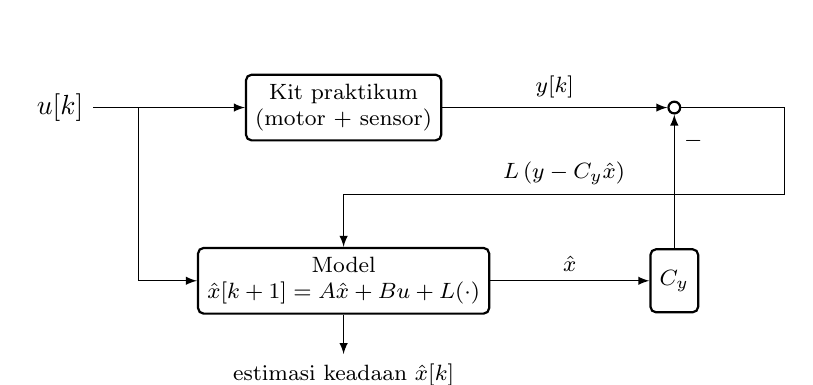
\begin{tikzpicture}[
blok/.style={draw, thick, rounded corners=2pt, minimum height=8mm, align=center, font=\footnotesize},
jum/.style={draw, thick, circle, inner sep=1.5pt},
>=latex]
\node[blok] (plant) at (0,0) {Kit praktikum\\(motor + sensor)};
\node[blok] (model) at (0,-2.2) {Model\\$\hat{x}[k+1] = A\hat{x} + Bu + L(\cdot)$};
\node[blok] (cy) at (4.2,-2.2) {$C_y$};
\node[jum] (s) at (4.2,0) {};
\node (u) at (-3.6,0) {$u[k]$};
\draw[->] (u) -- (plant);
\draw[->] (-2.6,0) |- (model);
\draw[->] (plant) -- node[above, font=\footnotesize] {$y[k]$} (s);
\draw[->] (model) -- node[above, font=\footnotesize] {$\hat{x}$} (cy);
\draw[->] (cy) -- node[right, font=\footnotesize, pos=0.8] {$-$} (s);
\draw[->] (s) -- ++(1.4,0) |- ++(0,-1.1) -| node[pos=0.25, above, font=\footnotesize] {$L\,(y - C_y\hat{x})$} (model.north);
\draw[->] (model.south) -- ++(0,-0.5) node[below, font=\footnotesize] {estimasi keadaan $\hat{x}[k]$};
\end{tikzpicture}
\caption{Struktur observer Luenberger}
\label{fig:observer}
\end{figure}

\paragraph{Observer A: kecepatan dari potensiometer.} Dengan $C_y = C_p = [1\;\;0]$, observer menggunakan bacaan posisi untuk memperkirakan posisi dan kecepatan. Karena bacaan posisi berpindah dari 100\% ke 0\%, selisih $y - C_y\hat{x}$ dibatasi dengan fungsi $\operatorname{wrap}$ seperti pada Modul 3, dan $\hat{p}$ dijaga pada rentang 0--100\%. Kecepatan perkiraan $\hat{v}$ memiliki tanda (arah putar) dan tetap tersedia pada kecepatan rendah ketika tachometer membaca nol.

\paragraph{Observer B: posisi dari tachometer.} Dengan $C_y = C_v = [0\;\;1]$, observer menggunakan bacaan kecepatan. Tachometer tidak membedakan arah putar, sehingga kecepatan bertanda didekati dengan
\begin{equation}
v_m = \operatorname{sign}(\text{arah perintah terakhir}) \times \text{bacaan tachometer},
\label{eq:kecepatan_bertanda}
\end{equation}
dengan arah diambil dari variabel \texttt{Direction} pada tab \prog{2\_actuator.ino}. Matriks $A - L C_v$ berbentuk segitiga atas dengan satu nilai eigen selalu di $z = 1$, berapa pun nilai $L$. Gain $L_{v1} = C\tau(1-a)$ membuat posisi perkiraan diperoleh dengan mengintegralkan kecepatan terukur (\textit{dead reckoning}), sedangkan $L_{v2} = a - z_v$ menempatkan kutub koreksi kecepatan di $z_v$. Posisi awal estimator diambil dari bacaan potensiometer saat program dimulai. Praktikan akan menyelidiki akibat sifat ini melalui pemeriksaan keteramatan dan percobaan.

\subsection{Prinsip Separasi}
Bila umpan balik keadaan menggunakan keadaan perkiraan, $u = -\mathbf{K}\hat{x}$, kutub sistem kalang tertutup gabungan adalah gabungan kutub $A - B\mathbf{K}$ dan kutub $A - LC_y$. Dengan demikian, pengontrol dan observer dapat dirancang secara terpisah. Prinsip ini berlaku untuk model linier yang tepat; ketidaktepatan model, waktu tunda, saturasi, dan \textit{deadzone} pada kit dapat membuat hasilnya berbeda.

\subsection{Implementasi pada Program}
Pada setiap waktu cacah, program \prog{11\_main\_state\_space} melakukan langkah berikut:
\begin{enumerate}
\item Membaca posisi $y_p[k]$ dan tachometer, lalu menghitung kecepatan bertanda $v_m[k]$.
\item Menghitung aksi kontrol $u[k]$ sesuai mode, menggunakan $\hat{x}[k]$ (bila observer dipakai) atau pengukuran langsung, lalu membatasinya.
\item Memberikan $u[k]$ ke motor melalui kompensasi \textit{deadzone}.
\item Memperbarui kedua observer dengan Persamaan~\eqref{eq:observer} untuk memperoleh $\hat{x}[k+1]$.
\end{enumerate}
Model menggunakan masukan sebelum kompensasi $u$, sama seperti model Modul 1. Matriks $A$ dan $B$ dihitung otomatis oleh fungsi \texttt{state\_space\_setup()} dari \texttt{ModelK}, \texttt{ModelTau}, \texttt{ModelC}, dan waktu cacah.

\section{Keselamatan Kerja}
Seluruh ketentuan keselamatan kerja dan SOP pada modul sebelumnya tetap berlaku. Perhatikan pula hal-hal berikut:
\begin{enumerate}
\item Periksa setiap gain hasil desain dengan simulasi sebelum diterapkan pada kit, dan verifikasi program tanpa daya motor.
\item Mulailah dengan kutub kontrol yang lambat. Kutub yang terlalu cepat dapat menyebabkan osilasi keras.
\item Pada Mode 0, urutan masukan harus melewati 0 sebelum berganti arah.
\item Bila motor berosilasi keras atau berputar tidak terkendali, segera cabut kabel listrik 220~V.
\end{enumerate}

\section{Prosedur Praktikum}
Prosedur Modul 4 terdiri atas lima percobaan. Simpan seluruh data mentah ke file teks.

\subsection{Percobaan 1: Model Ruang Keadaan dan Desain}
\begin{enumerate}
\item Isi parameter model dan waktu cacah pada skrip \prog{desain\_state\_space.m}. Gunakan waktu cacah pertama dari Modul 1 atau waktu cacah lain yang dijustifikasi.
\item Jalankan skrip dan lengkapi Tabel~\ref{tab:p1_model} dengan matriks $A$ dan $B$, pangkat matriks keterkendalian, serta pangkat matriks keteramatan untuk kedua keluaran.
\item Tentukan dua set spesifikasi kontrol posisi (Desain 1 lebih lambat, Desain 2 lebih cepat), satu set spesifikasi kontrol kecepatan, dan spesifikasi observer. Catat gain dan kutub hasil desain pada Tabel~\ref{tab:p1_gain}.
\item Amati grafik simulasi yang dihasilkan skrip. Pastikan simulasi stabil dan aksi kontrol tidak terus-menerus saturasi sebelum gain diterapkan pada kit.
\end{enumerate}

\begin{table}[H]
\centering
\caption{Model ruang keadaan diskrit kit praktikum}
\label{tab:p1_model}
\begin{tabularx}{\textwidth}{|l|X|}
\hline
\textbf{Besaran} & \textbf{Nilai} \\
\hline
$K$, $\tau$ (ms), $\theta$ (ms), $C$, $T_s$ (ms) & \\
Matriks $A$ & \\
Matriks $B$ & \\
Pangkat $W_c$ & \\
Pangkat $W_o$ dengan $C_p = [1\;\;0]$ & \\
Pangkat $W_o$ dengan $C_v = [0\;\;1]$ & \\
\hline
\end{tabularx}
\end{table}

\begin{table}[H]
\centering
\caption{Spesifikasi, kutub, dan gain hasil desain}
\label{tab:p1_gain}
\small
\begin{tabularx}{\textwidth}{|l|X|X|X|}
\hline
\textbf{Desain} & \textbf{Spesifikasi} & \textbf{Kutub diskrit} & \textbf{Gain} \\
\hline
Kecepatan & $\tau_c$ = & $z_c$ = & $k_v$ = \quad $N$ = \\
Posisi, Desain 1 & $\zeta$ = \quad $t_s$ = & & $k_1$ = \quad $k_2$ = \\
Posisi, Desain 2 & $\zeta$ = \quad $t_s$ = & & $k_1$ = \quad $k_2$ = \\
Observer A & $\zeta$ = \quad $t_s$ = & & $L_{p1}$ = \quad $L_{p2}$ = \\
Observer B & $\tau_v$ = & & $L_{v1}$ = \quad $L_{v2}$ = \\
\hline
\end{tabularx}
\end{table}

\subsection{Percobaan 2: Pole Placement Kecepatan}
\begin{enumerate}
\item Ganti tab \prog{9\_main.ino} dengan program \prog{11\_main\_state\_space} (Kode~\ref{lst:main}). Salin baris hasil skrip ke \texttt{setup()}, atur \texttt{TimeSampling} sesuai desain, \texttt{Mode = 1}, dan \texttt{Sequence = \{0, 40, 70, 30, 0\}}.
\item Verifikasi tanpa daya motor bahwa $U = N r$ ketika kecepatan nol, lalu jalankan dengan daya motor dan simpan datanya.
\item Ulangi dengan konstanta waktu kalang tertutup lain (misalnya $\tau_c$ dua kali lebih kecil).
\item Untuk setiap perubahan set point, ukur konstanta waktu kalang tertutup (waktu mencapai 63,2\% perubahan) dan offset. Lengkapi Tabel~\ref{tab:p2_kecepatan}.
\end{enumerate}

\begin{table}[H]
\centering
\caption{Performa pole placement kecepatan}
\label{tab:p2_kecepatan}
\begin{tabularx}{\textwidth}{|c|c|C|C|C|}
\hline
\textbf{$\tau_c$ desain (ms)} & \textbf{Step} & \textbf{$\tau_c$ terukur (ms)} & \textbf{Offset (\%)} & \textbf{$u$ maksimum (\%)} \\
\hline
\multirow{3}{*}{} & $0 \rightarrow 40$ & & & \\
\cline{2-5}
& $40 \rightarrow 70$ & & & \\
\cline{2-5}
& $70 \rightarrow 30$ & & & \\
\hline
\multirow{3}{*}{} & $0 \rightarrow 40$ & & & \\
\cline{2-5}
& $40 \rightarrow 70$ & & & \\
\cline{2-5}
& $70 \rightarrow 30$ & & & \\
\hline
\end{tabularx}
\end{table}

\subsection{Percobaan 3: Uji Observer pada Kalang Terbuka}
\begin{enumerate}
\item Atur \texttt{Mode = 0}. Pilih masukan kecil $u_{kecil}$ yang membuat motor berputar pelan tetapi tachometer masih membaca nol atau hampir nol (lihat spesifikasi kit pada Modul 1). Atur \texttt{Sequence = \{0, }$u_{kecil}$\texttt{, 0, 30, 0, -30, 0, 60, 0, -60, 0\}}.
\item Verifikasi tanpa daya motor, lalu jalankan dan simpan data ke file \prog{data\_observer.txt}. Program mencetak posisi terukur, posisi perkiraan observer A (\texttt{PosHat}), posisi perkiraan observer B (\texttt{PosHatT}), kecepatan bertanda dari tachometer (\texttt{VelT}), kecepatan perkiraan observer A (\texttt{VelHat}), dan masukan.
\item Jalankan skrip \prog{analisis\_observer.m} (Kode~\ref{lst:analisis}) untuk membandingkan $\hat{v}$ dengan kecepatan tachometer dan dengan turunan numerik posisi, serta $\hat{p}$ observer B dengan posisi terukur.
\item Ulangi dengan observer A yang lebih lambat dan yang lebih cepat (ubah \texttt{TsObs} pada skrip desain, lalu salin gain baru). Lengkapi Tabel~\ref{tab:p3_observer}.
\item \textbf{Uji simpangan observer B}: jalankan urutan yang lebih panjang (misalnya ulangi urutan masukan dua hingga tiga kali). Catat error posisi observer B pada awal dan akhir percobaan.
\end{enumerate}

\begin{table}[H]
\centering
\caption{Hasil uji observer pada kalang terbuka}
\label{tab:p3_observer}
\small
\begin{tabularx}{\textwidth}{|c|C|C|C|C|C|}
\hline
\textbf{Observer A ($t_s$ obs.)} & \textbf{RMSE $\hat{v}$ vs tachometer (\%)} & \textbf{RMSE turunan numerik (\%)} & \textbf{$\hat{v}$ pada $u_{kecil}$ (\%)} & \textbf{Error $\hat{p}_B$ awal (\%)} & \textbf{Error $\hat{p}_B$ akhir (\%)} \\
\hline
 & & & & & \\
\hline
 & & & & & \\
\hline
 & & & & & \\
\hline
\end{tabularx}
\end{table}

\subsection{Percobaan 4: Pole Placement Posisi dengan Observer}
\begin{enumerate}
\item Atur \texttt{Mode = 2}, \texttt{UseObserver = true}, batas \texttt{UMax} sesuai Modul 3, gain Desain 1, dan \texttt{Sequence = \{50, 20, 50, 90, 20, 50\}}.
\item Verifikasi tanpa daya motor, lalu jalankan dan simpan datanya. Hitung performa untuk perubahan set point $50 \rightarrow 20$ dan $20 \rightarrow 50$.
\item Ulangi dengan gain Desain 2.
\item Ulangi Desain 1 dengan \texttt{UseObserver = false}, sehingga kecepatan umpan balik diambil dari tachometer bertanda.
\item Lengkapi Tabel~\ref{tab:p4_posisi}. Tambahkan pengontrol posisi terbaik dari Modul 3 sebagai pembanding.
\item \textbf{Uji gangguan}: dengan desain terbaik, setelah urutan selesai set point terakhir dipertahankan. Berikan gangguan dengan memutar roda gigi potensiometer sedikit, lalu lepaskan. Simpan responsnya.
\end{enumerate}

\begin{table}[H]
\centering
\caption{Performa pole placement posisi}
\label{tab:p4_posisi}
\small
\begin{tabularx}{\textwidth}{|l|c|C|C|C|C|C|}
\hline
\textbf{Pengontrol} & \textbf{Step} & \textbf{$t_d$ (ms)} & \textbf{$t_r$ (ms)} & \textbf{$M_p$ (\%)} & \textbf{$t_s$ (ms)} & \textbf{Offset (\%)} \\
\hline
\multirow{2}{*}{Desain 1, observer} & $50 \rightarrow 20$ & & & & & \\
\cline{2-7}
& $20 \rightarrow 50$ & & & & & \\
\hline
\multirow{2}{*}{Desain 2, observer} & $50 \rightarrow 20$ & & & & & \\
\cline{2-7}
& $20 \rightarrow 50$ & & & & & \\
\hline
\multirow{2}{*}{Desain 1, tachometer} & $50 \rightarrow 20$ & & & & & \\
\cline{2-7}
& $20 \rightarrow 50$ & & & & & \\
\hline
\multirow{2}{*}{Terbaik Modul 3} & $50 \rightarrow 20$ & & & & & \\
\cline{2-7}
& $20 \rightarrow 50$ & & & & & \\
\hline
\end{tabularx}
\end{table}

\subsection{Percobaan 5: Perbandingan dengan Simulasi}
\begin{enumerate}
\item Pada skrip \prog{desain\_state\_space.m}, ubah urutan set point simulasi agar sama dengan percobaan, lalu bandingkan respons simulasi dengan respons kit untuk Desain 1 dan Desain 2.
\item Pada simulasi, ubah waktu tunda \texttt{Theta} menjadi nol dan dua kali nilai sebenarnya. Amati pengaruh waktu tunda terhadap respons pole placement.
\end{enumerate}

\section{Laporan dan Analisis}
\subsection{Ketentuan Laporan}
% TODO: sesuaikan platform dan tenggat pengumpulan
Laporan dikumpulkan per kelompok melalui Edunex paling lambat dua minggu setelah praktikum. Nilai tambahan diberikan bila laporan dikumpulkan dalam satu minggu. Laporan berupa file \texttt{.pdf} yang dilampiri \textit{spreadsheet} pengolahan data, data mentah (\texttt{.txt}), program Arduino, dan skrip MATLAB, digabung dalam satu file \texttt{.zip}. Laporan minimal memiliki susunan berikut: latar belakang, tujuan, alat, prosedur, analisis, kesimpulan, kontribusi, dan referensi.

Latar belakang, tujuan, alat, dan prosedur tidak boleh sama persis dengan modul ini. Analisis disusun dengan alur yang runtut dengan menjawab pertanyaan pada Bagian~\ref{sec:analisis}. Perhatikan penggunaan angka penting. Bagian kontribusi berisi Tabel~\ref{tab:kontribusi}.

\begin{table}[H]
\centering
\caption{Kontribusi anggota kelompok}
\label{tab:kontribusi}
\begin{tabularx}{\textwidth}{|c|c|l|X|}
\hline
\textbf{No} & \textbf{NIM} & \textbf{Nama Lengkap} & \textbf{Kontribusi} \\
\hline
1 & & & \\
2 & & & \\
3 & & & \\
4 & & & \\
5 & & & \\
\hline
\end{tabularx}
\end{table}

\subsection{Analisis}
\label{sec:analisis}

\paragraph{Model ruang keadaan.}
\begin{enumerate}
\item Turunkan Persamaan~\eqref{eq:ss_diskrit} dari Persamaan~\eqref{eq:ss_kontinu}. Tunjukkan bahwa baris kedua sama dengan model diskrit kecepatan pada Modul 1.
\item Apakah sistem terkendali? Apakah sistem teramati dari potensiometer? Apakah sistem teramati dari tachometer? Jelaskan arti fisis hasil tersebut.
\item Di mana letak kutub sistem kalang terbuka? Apa arti kutub di $z = 1$?
\end{enumerate}

\paragraph{Pole placement kecepatan.}
\begin{enumerate}[resume]
\item Bandingkan konstanta waktu kalang tertutup terukur dengan desain. Bila berbeda, apa penyebabnya?
\item Apakah terdapat offset? Jelaskan penyebabnya dan usulkan cara menghilangkannya tanpa mengubah kutub yang dirancang.
\item Bandingkan pole placement kecepatan dengan pengontrol terbaik Modul 2 dari segi kecepatan respons, offset, dan kemudahan perancangan.
\end{enumerate}

\paragraph{Observer.}
\begin{enumerate}[resume]
\item Bandingkan $\hat{v}$ observer A dengan kecepatan tachometer dan dengan turunan numerik posisi. Mana yang paling halus, dan mana yang paling akurat? Jelaskan.
\item Apa yang terlihat pada $\hat{v}$ ketika masukan $u_{kecil}$ diberikan? Apa keunggulan observer A dibandingkan tachometer pada kondisi ini dan saat motor berbalik arah?
\item Bagaimana pengaruh kecepatan kutub observer A terhadap derau dan keterlambatan estimasi? Bagaimana memilih kutub observer yang baik?
\item Apakah terdapat selisih tetap antara $\hat{p}$ observer A dan posisi terukur ketika motor berputar dengan kecepatan konstan? Kaitkan dengan waktu tunda yang diabaikan pada model.
\item Tunjukkan error posisi observer B terhadap waktu. Apakah error konvergen ke nol? Jelaskan hasilnya berdasarkan pemeriksaan keteramatan dan nilai eigen $A - LC_v$.
\item Sebutkan sumber-sumber error estimasi posisi dari tachometer (misalnya tanda kecepatan, kecepatan rendah, filter tachometer, dan ketidaktepatan $C$). Mana yang paling dominan pada percobaan?
\item Bagaimana estimasi posisi dari tachometer dapat diperbaiki bila potensiometer tetap tersedia? Kaitkan jawaban dengan observer A.
\end{enumerate}

\paragraph{Pole placement posisi dengan observer.}
\begin{enumerate}[resume]
\item Bandingkan respons Desain 1 dan Desain 2 dengan spesifikasi desain dan dengan simulasi. Apakah kutub yang lebih cepat selalu menghasilkan respons yang lebih baik pada kit?
\item Bandingkan umpan balik kecepatan dari observer dan dari tachometer bertanda. Mana yang lebih baik, dan mengapa?
\item Bandingkan pole placement posisi dengan pengontrol terbaik Modul 3. Kaitkan struktur $u = -k_1 e - k_2 v$ dengan pengontrol PD.
\item Bagaimana respons terhadap gangguan manual? Apakah observer tetap memberikan estimasi yang baik selama gangguan?
\item Berdasarkan simulasi dengan waktu tunda yang berbeda, seberapa besar pengaruh waktu tunda yang diabaikan pada desain?
\end{enumerate}

\section{Tugas Tambahan}
Tugas tambahan bersifat opsional dan dapat ditambahkan pada laporan untuk nilai tambah.
\begin{enumerate}
\item Tambahkan keadaan integral error, $x_I[k+1] = x_I[k] + (r - v[k])$, pada kontrol kecepatan, lalu rancang pole placement untuk sistem orde dua hasil augmentasi. Apakah offset hilang?
\item Masukkan waktu tunda ke dalam model dengan menambahkan keadaan $u[k-1], \ldots, u[k-d]$. Rancang ulang pengontrol dan observer, lalu bandingkan hasilnya.
\item Rancang observer A dengan filter Kalman (gain tunak) berdasarkan variansi derau potensiometer dan model. Bandingkan dengan observer hasil pole placement.
\item Gunakan observer orde penuh dengan dua keluaran (posisi dan kecepatan) sekaligus. Bagaimana memilih gain $L$ berukuran $2 \times 2$?
\end{enumerate}

\begin{thebibliography}{9}
\bibitem{ogata_d} K.~Ogata, \textit{Discrete-Time Control Systems}, edisi ke-2. Upper Saddle River, NJ: Prentice Hall, 1995.
\bibitem{astrom} K.~J. Åström dan B.~Wittenmark, \textit{Computer-Controlled Systems: Theory and Design}, edisi ke-3. Englewood Cliffs, NJ: Prentice Hall, 1997.
\bibitem{franklin} G.~F. Franklin, J.~D. Powell, dan M.~L. Workman, \textit{Digital Control of Dynamic Systems}, edisi ke-3. Menlo Park, CA: Addison-Wesley, 1998.
\end{thebibliography}

\clearpage
\appendix
\section{Kode Program Pendukung}
\label{lamp:kode}
Tab \prog{6\_state\_space.ino} ditambahkan ke folder program. Program utama \prog{11\_main\_state\_space} menggantikan isi tab \prog{9\_main.ino}. Tab lain tetap sama seperti pada Modul 3.

\begin{lstlisting}[caption={Tab \texttt{6\_state\_space.ino}},label={lst:ss}]
// ===========================================================================
// Tab ruang keadaan (Modul 4): model diskrit, umpan balik keadaan, observer
//
// Keadaan x = [posisi (%); kecepatan bertanda (%)], masukan u (%).
// Model diskrit (ZOH, waktu tunda diabaikan):
//   x[k+1] = A x[k] + B u[k]
//   A = [1  A12; 0  A22],  B = [B1; B2]
// Parameter model berasal dari Modul 1 (ModelK, ModelTau) dan Modul 3
// (ModelC). Gain dihitung dengan skrip desain_state_space.m.
// ===========================================================================

// Parameter model (Tau dalam ms, C dalam %/ms per % kecepatan)
float ModelK = 0.85, ModelTau = 60.0, ModelC = 0.02;
float A12 = 0.0, A22 = 0.0, B1 = 0.0, B2 = 0.0;

// Pole placement kecepatan (satu keadaan): u = Nspeed*r - Kspeed*v
float Kspeed = 0.0, Nspeed = 1.0;

// Pole placement posisi (dua keadaan): u = -(Kpos*(p - r) + Kvel*v)
float Kpos = 0.5, Kvel = 0.25;

// Observer A: keluaran terukur posisi (potensiometer) -> estimasi kecepatan
float Lp1 = 0.5, Lp2 = 0.4;
float PosHat = 0.0, VelHat = 0.0;

// Observer B: keluaran terukur kecepatan (tachometer) -> estimasi posisi
float Lv1 = 0.0, Lv2 = 0.0;
float PosHatT = 0.0, VelHatT = 0.0;

void state_space_setup(unsigned int Ts) {
  float a = exp(-(float) Ts / ModelTau);
  A12 = ModelC * ModelTau * (1.0 - a);
  A22 = a;
  B1 = ModelC * ModelK * ((float) Ts - ModelTau * (1.0 - a));
  B2 = ModelK * (1.0 - a);
}

float wrap_error(float e) {
  while (e > 50.0) e -= 100.0;
  while (e < -50.0) e += 100.0;
  return e;
}

float wrap_position(float p) {
  while (p >= 100.0) p -= 100.0;
  while (p < 0.0) p += 100.0;
  return p;
}

void observer_reset(float Position, float Velocity) {
  PosHat = Position;
  VelHat = Velocity;
  PosHatT = Position;
  VelHatT = Velocity;
}

// Dipanggil sekali setiap waktu cacah, setelah masukan u[k] diberikan.
// Menghasilkan estimasi keadaan untuk cacah berikutnya, x_hat[k+1].
void observer_update(float PositionMeasured, float VelocityMeasured, float U) {
  // Observer A: koreksi berdasarkan error posisi (dibatasi -50 hingga 50)
  float Innovation = wrap_error(PositionMeasured - PosHat);
  float NextPos = PosHat + A12 * VelHat + B1 * U + Lp1 * Innovation;
  float NextVel = A22 * VelHat + B2 * U + Lp2 * Innovation;
  PosHat = wrap_position(NextPos);
  VelHat = NextVel;

  // Observer B: koreksi berdasarkan error kecepatan
  float InnovationT = VelocityMeasured - VelHatT;
  float NextPosT = PosHatT + A12 * VelHatT + B1 * U + Lv1 * InnovationT;
  float NextVelT = A22 * VelHatT + B2 * U + Lv2 * InnovationT;
  PosHatT = wrap_position(NextPosT);
  VelHatT = NextVelT;
}
\end{lstlisting}

\begin{lstlisting}[caption={Program utama \texttt{11\_main\_state\_space}},label={lst:main}]
// ===========================================================================
// Program utama Modul 4: pole placement dan observer
// Ganti isi tab 9_main.ino dengan program ini. Tab 6_state_space.ino harus
// sudah ditambahkan.
//
// Mode = 0 : kalang terbuka. Sequence[] berisi masukan motor (%). Digunakan
//            untuk menguji kedua observer.
// Mode = 1 : pole placement kecepatan. Sequence[] berisi set point kecepatan
//            (%, positif saja).
// Mode = 2 : pole placement posisi. Sequence[] berisi set point posisi (%).
//            Kecepatan umpan balik dari observer (UseObserver = true) atau
//            dari tachometer bertanda (UseObserver = false). Setelah urutan
//            selesai, set point terakhir dipertahankan.
// ===========================================================================

unsigned long Time, StartTime, LastTime, StepStart;
unsigned int TimeSampling = 10, DeltaTime;   // waktu cacah (ms)
unsigned int HoldTime = 3000;                // lama tiap nilai Sequence (ms)
byte Mode = 0;
bool UseObserver = true;
float UMax = 40.0;                           // batas masukan pada Mode 2 (%)

float Sequence[] = {0, 30, 0, -30, 0, 60, 0, -60, 0};
const byte SequenceLength = sizeof(Sequence) / sizeof(Sequence[0]);

byte Index = 0;
float Reference = 0.0, PositionMeasured = 0.0, Tacho = 0.0;
float SpeedSign = 1.0, VelocitySigned = 0.0, U = 0.0, Motor = 0.0;
bool Finished = false;

void setup() {
  general_setup();
  sensor_setup();
  actuator_setup();

  // Parameter model dan gain hasil desain_state_space.m
  ModelK = 0.85;  ModelTau = 60.0;  ModelC = 0.02;
  Kspeed = 0.0;   Nspeed = 1.0;
  Kpos = 0.5;     Kvel = 0.25;
  Lp1 = 0.5;      Lp2 = 0.4;
  Lv1 = 0.0;      Lv2 = 0.0;

  state_space_setup(TimeSampling);
  observer_reset(smooth_position_percentage(), 0.0);

  Serial.println("Time\tDelta\tRef\tPos\tPosHat\tPosHatT\tVelT\tVelHat\tU");
  StartTime = millis();
  LastTime = StartTime;
  StepStart = StartTime;
}

void loop() {
  Time = millis();
  if (Time - LastTime >= TimeSampling) {
    DeltaTime = Time - LastTime;
    LastTime = Time;

    Reference = Sequence[Index];
    PositionMeasured = smooth_position_percentage();
    Tacho = smooth_velocity_percentage();

    // Tachometer tidak membedakan arah: tanda diambil dari arah putar
    // terakhir yang diperintahkan ke driver (variabel Direction).
    if (Direction != 0) SpeedSign = (float) Direction;
    VelocitySigned = SpeedSign * Tacho;

    if (Finished && Mode != 2) {
      U = 0.0;
    }
    else if (Mode == 0) {
      U = Reference;
    }
    else if (Mode == 1) {
      if (Reference <= 0.0) U = 0.0;
      else U = Nspeed * Reference - Kspeed * Tacho;
      if (U > 100.0) U = 100.0;
      if (U < 0.0) U = 0.0;
    }
    else {
      float Velocity = UseObserver ? VelHat : VelocitySigned;
      U = -(Kpos * wrap_error(PositionMeasured - Reference) + Kvel * Velocity);
      if (U > UMax) U = UMax;
      if (U < -UMax) U = -UMax;
    }

    Motor = run_motor(compensation(U));
    if (Motor == 0.0 && U != 0.0) U = 0.0;   // satu cacah pengereman saat arah berbalik
    observer_update(PositionMeasured, VelocitySigned, U);

    Serial.print(Time - StartTime);
    Serial.print("\t");
    Serial.print(DeltaTime);
    Serial.print("\t");
    Serial.print(Reference);
    Serial.print("\t");
    Serial.print(PositionMeasured);
    Serial.print("\t");
    Serial.print(PosHat);
    Serial.print("\t");
    Serial.print(PosHatT);
    Serial.print("\t");
    Serial.print(VelocitySigned);
    Serial.print("\t");
    Serial.print(VelHat);
    Serial.print("\t");
    Serial.println(U);

    if (!Finished && Time - StepStart >= HoldTime) {
      StepStart = Time;
      if (Index < SequenceLength - 1) Index++;
      else Finished = true;
    }
  }
}
\end{lstlisting}

\begin{lstlisting}[language=Matlab, morekeywords={yline,stairs,eig,poly,rank,mat2str,struct,conj}, caption={Skrip MATLAB \texttt{desain\_state\_space.m}},label={lst:desain}]
%% desain_state_space.m
% Desain pole placement dan observer untuk kit praktikum SKD (Modul 4).
%
% Keadaan x = [posisi (%); kecepatan bertanda (%)], masukan u (%).
% Model diskrit (ZOH, waktu tunda diabaikan pada desain):
%   x[k+1] = A x[k] + B u[k]
%   A = [1, C*Tau*(1-a); 0, a],  B = [C*K*(Ts - Tau*(1-a)); K*(1-a)],  a = exp(-Ts/Tau)
%
% Skrip ini:
%   1. menghitung A dan B, keterkendalian, dan keteramatan,
%   2. menghitung gain pole placement kecepatan (1 keadaan) dan posisi (2 keadaan),
%   3. menghitung gain observer kecepatan dari potensiometer (observer A)
%      dan estimator posisi dari tachometer (observer B),
%   4. mensimulasikan sistem dengan waktu tunda, saturasi, dan derau sensor,
%   5. menampilkan baris program untuk disalin ke 11_main_state_space.ino.

clc; clear; close all;

%% 1. Parameter model (waktu dalam ms)
K     = 0.85;     % penguatan (Modul 1)
Tau   = 60;       % konstanta waktu (ms) (Modul 1)
Theta = 30;       % waktu tunda (ms) (Modul 1), hanya untuk simulasi
C     = 0.02;     % konversi kecepatan ke laju posisi (%/ms per %) (Modul 3)
Ts    = 10;       % waktu cacah (ms)
UMax  = 40;       % batas masukan kontrol posisi (%)

%% 2. Spesifikasi desain
TauSpeed = 30;    % konstanta waktu kalang tertutup kontrol kecepatan (ms)
Zeta     = 0.8;   % rasio redaman kontrol posisi
TsPos    = 400;   % settling time 2% kontrol posisi (ms)
ZetaObs  = 0.8;   % rasio redaman observer A
TsObs    = 100;   % settling time observer A (ms), lebih cepat dari kontrol
TauObsV  = 20;    % konstanta waktu koreksi kecepatan observer B (ms)

%% 3. Model diskrit, keterkendalian, dan keteramatan
a = exp(-Ts/Tau);
A = [1, C*Tau*(1 - a); 0, a];
B = [C*K*(Ts - Tau*(1 - a)); K*(1 - a)];
Cpos = [1 0];     % keluaran potensiometer
Cvel = [0 1];     % keluaran tachometer
Wc   = [B, A*B];
WoP  = [Cpos; Cpos*A];
WoV  = [Cvel; Cvel*A];
fprintf('A = [%.5f %.5f; %.5f %.5f],  B = [%.6f; %.6f]\n', A', B);
fprintf('Rank matriks keterkendalian           : %d\n', rank(Wc));
fprintf('Rank matriks keteramatan (posisi)     : %d\n', rank(WoP));
fprintf('Rank matriks keteramatan (kecepatan)  : %d\n', rank(WoV));

%% 4. Pole placement kecepatan: u = Nspeed*r - Kspeed*v
zSpeed = exp(-Ts/TauSpeed);
Kspeed = (a - zSpeed) / B(2);
Nspeed = (1 - zSpeed) / B(2);

%% 5. Pole placement posisi: u = -(Kpos*(p - r) + Kvel*v)
zCtrl = kutub_diskrit(Zeta, TsPos, Ts);
Kf = ackermann(A, B, zCtrl);
Kpos = Kf(1); Kvel = Kf(2);

%% 6. Observer A (posisi terukur) dan observer B (kecepatan terukur)
zObs = kutub_diskrit(ZetaObs, TsObs, Ts);
Lp = ackermann(A', Cpos', zObs)';      % dualitas: L = acker(A', C', p)'
zVel = exp(-Ts/TauObsV);
Lv = [A(1,2); a - zVel];               % Lv1 = A12: posisi = integral kecepatan terukur

fprintf('\nKutub kontrol posisi : %s\n', mat2str(eig(A - B*Kf).', 4));
fprintf('Kutub observer A     : %s\n', mat2str(eig(A - Lp*Cpos).', 4));
fprintf('Kutub observer B     : %s\n', mat2str(eig(A - Lv*Cvel).', 4));

fprintf('\n// ---- salin ke setup() pada 11_main_state_space.ino ----\n');
fprintf('ModelK = %.4f;  ModelTau = %.2f;  ModelC = %.5f;\n', K, Tau, C);
fprintf('Kspeed = %.4f;  Nspeed = %.4f;\n', Kspeed, Nspeed);
fprintf('Kpos = %.4f;  Kvel = %.4f;\n', Kpos, Kvel);
fprintf('Lp1 = %.4f;  Lp2 = %.4f;\n', Lp(1), Lp(2));
fprintf('Lv1 = %.4f;  Lv2 = %.4f;\n', Lv(1), Lv(2));
fprintf('// TimeSampling = %g;\n', Ts);

%% 7. Simulasi
Prm = struct('K', K, 'Tau', Tau, 'Theta', Theta, 'C', C, 'Ts', Ts, 'UMax', UMax, ...
    'Kspeed', Kspeed, 'Nspeed', Nspeed, 'Kpos', Kpos, 'Kvel', Kvel, 'Lp', Lp, 'Lv', Lv, ...
    'A', A, 'B', B, 'TachoMin', 3, 'Derau', 0.5);

% (a) Kalang terbuka: uji kedua observer
S = simulasi(Prm, 0, [0 30 0 -30 0 60 0 -60 0], 3000, true);
figure('Name', 'Observer (kalang terbuka)');
subplot(2,1,1); plot(S.t, S.v, 'k', S.t, S.vT, 'b.', S.t, S.vHat, 'r'); grid on;
legend('Kecepatan sebenarnya', 'Tachometer bertanda', 'Estimasi observer A');
ylabel('Kecepatan (%)');
subplot(2,1,2); plot(S.t, S.pTrue, 'k', S.t, S.pHatT, 'r'); grid on;
legend('Posisi sebenarnya (tanpa batas)', 'Estimasi observer B');
xlabel('Waktu (ms)'); ylabel('Posisi (%)');

% (b) Pole placement kecepatan
S = simulasi(Prm, 1, [0 40 70 30 0], 1500, true);
figure('Name', 'Pole placement kecepatan');
stairs(S.t, S.r, 'k--'); hold on; plot(S.t, S.v, 'b'); grid on;
xlabel('Waktu (ms)'); ylabel('Kecepatan (%)'); legend('Set point', 'Kecepatan');

% (c) Pole placement posisi: observer vs tachometer bertanda
Ref = [50 20 50 90 20 50];
S1 = simulasi(Prm, 2, Ref, 2000, true);
S2 = simulasi(Prm, 2, Ref, 2000, false);
figure('Name', 'Pole placement posisi');
stairs(S1.t, S1.r, 'k--'); hold on;
plot(S1.t, S1.p, 'b', S2.t, S2.p, 'r'); grid on;
xlabel('Waktu (ms)'); ylabel('Posisi (%)');
legend('Set point', 'Umpan balik observer', 'Umpan balik tachometer');

%% Fungsi bantu
function z = kutub_diskrit(Zeta, TSettle, Ts)
    % Pasangan kutub diskrit dari rasio redaman dan settling time 2%
    wn = 4 / (Zeta * TSettle);
    s  = -Zeta*wn + 1i*wn*sqrt(1 - Zeta^2);
    z  = exp([s; conj(s)] * Ts);
end

function Kg = ackermann(A, B, Kutub)
    % Rumus Ackermann untuk sistem orde dua
    al  = real(poly(Kutub));               % [1 alpha1 alpha0]
    Phi = A^2 + al(2)*A + al(3)*eye(2);
    Kg  = [0 1] / [B, A*B] * Phi;
end

function S = simulasi(Prm, Mode, Seq, Hold, PakaiObserver)
    % Plant kontinu (langkah 1 ms) dengan waktu tunda, saturasi, dan derau.
    Ts = Prm.Ts; d = round(Prm.Theta); N = Hold * numel(Seq);
    ubuf = zeros(N + d + 1, 1);
    v = 0; p = 50; u = 0; Arah = 1;
    xA = [50; 0]; xB = [50; 0];
    nk = floor((N - 1)/Ts) + 1;
    S = struct('t', zeros(nk,1), 'r', zeros(nk,1), 'v', zeros(nk,1), 'vT', zeros(nk,1), ...
        'vHat', zeros(nk,1), 'p', zeros(nk,1), 'pTrue', zeros(nk,1), 'pHatT', zeros(nk,1));
    i = 0;
    for k = 0:N-1
        if mod(k, Ts) == 0
            r = Seq(min(numel(Seq), floor(k/Hold) + 1));
            pm = mod(p + 0.1*randn, 100);                    % potensiometer
            vt = abs(v); if vt < Prm.TachoMin, vt = 0; end   % tachometer
            vt = max(0, vt + Prm.Derau*randn*(vt > 0));
            if u ~= 0, Arah = sign(u); end
            vs = Arah * vt;
            switch Mode
                case 0
                    u = r;
                case 1
                    if r <= 0, u = 0; else, u = Prm.Nspeed*r - Prm.Kspeed*vt; end
                    u = min(100, max(0, u));
                otherwise
                    if PakaiObserver, vf = xA(2); else, vf = vs; end
                    u = -(Prm.Kpos*bungkus(pm - r) + Prm.Kvel*vf);
                    u = min(Prm.UMax, max(-Prm.UMax, u));
            end
            % observer A (posisi terukur) dan observer B (kecepatan terukur)
            xA = Prm.A*xA + Prm.B*u + Prm.Lp*bungkus(pm - xA(1)); xA(1) = mod(xA(1), 100);
            xB = Prm.A*xB + Prm.B*u + Prm.Lv*(vs - xB(2));
            i = i + 1;
            S.t(i) = k; S.r(i) = r; S.v(i) = v; S.vT(i) = vs; S.vHat(i) = xA(2);
            S.p(i) = pm; S.pTrue(i) = p; S.pHatT(i) = xB(1);
        end
        ubuf(k + 1 + d) = u;
        v = v + (Prm.K*ubuf(k + 1) - v) / Prm.Tau;
        p = p + Prm.C * v;
    end
end

function e = bungkus(e)
    % Membatasi error posisi pada rentang -50 hingga 50
    e = mod(e + 50, 100) - 50;
end
\end{lstlisting}

\begin{lstlisting}[language=Matlab, morekeywords={readmatrix}, caption={Skrip MATLAB \texttt{analisis\_observer.m}},label={lst:analisis}]
%% analisis_observer.m
% Analisis data percobaan observer (Modul 4) dari program 11_main_state_space.
% Kolom data: Time | Delta | Ref | Pos | PosHat | PosHatT | VelT | VelHat | U

clc; clear; close all;

NamaFile = 'data_observer.txt';
C  = 0.02;          % konversi kecepatan ke laju posisi (%/ms per %), dari Modul 3
VelMin = 5;         % batas kecepatan (%) untuk membandingkan estimasi dengan tachometer

Data = readmatrix(NamaFile);
Data = Data(all(~isnan(Data(:, 1:9)), 2), :);
t      = Data(:,1) - Data(1,1);
Ref    = Data(:,3);
Pos    = Data(:,4);
PosHat = Data(:,5);
PosHatT= Data(:,6);
VelT   = Data(:,7);
VelHat = Data(:,8);
U      = Data(:,9);

% Posisi tanpa batas 0-100 (unwrap dengan periode 100%)
PosU     = buka(Pos);
PosHatTU = buka(PosHatT);

% Kecepatan dari turunan numerik posisi (pembanding sederhana)
VelDiff = [0; diff(PosU) ./ diff(t)] / C;

%% Observer A: estimasi kecepatan dari potensiometer
Bergerak = abs(VelT) > VelMin;
RMSE_A = sqrt(mean((VelHat(Bergerak) - VelT(Bergerak)).^2));
RMSE_D = sqrt(mean((VelDiff(Bergerak) - VelT(Bergerak)).^2));
fprintf('RMSE kecepatan observer A terhadap tachometer : %.2f %%\n', RMSE_A);
fprintf('RMSE kecepatan turunan numerik posisi        : %.2f %%\n', RMSE_D);

figure('Name', 'Observer A');
plot(t, VelT, 'b.', t, VelDiff, 'Color', [0.6 0.6 0.6]); hold on;
plot(t, VelHat, 'r', 'LineWidth', 1.2); grid on;
xlabel('Waktu (ms)'); ylabel('Kecepatan (%)');
legend('Tachometer bertanda', 'Turunan numerik posisi', 'Estimasi observer A');

%% Observer B: estimasi posisi dari tachometer
ErrB = PosHatTU - PosU;
fprintf('Error posisi observer B: awal %.2f %%, akhir %.2f %%, maksimum %.2f %%\n', ...
    ErrB(1), ErrB(end), max(abs(ErrB)));

figure('Name', 'Observer B');
subplot(2,1,1); plot(t, PosU, 'k', t, PosHatTU, 'r'); grid on;
ylabel('Posisi (%, tanpa batas)'); legend('Potensiometer', 'Estimasi observer B');
subplot(2,1,2); plot(t, ErrB, 'r'); grid on;
xlabel('Waktu (ms)'); ylabel('Error posisi (%)');

%% Fungsi bantu
function y = buka(x)
    % unwrap posisi dengan periode 100%
    y = x;
    for k = 2:numel(x)
        dx = x(k) - x(k-1);
        dx = mod(dx + 50, 100) - 50;
        y(k) = y(k-1) + dx;
    end
end
\end{lstlisting}

\end{document}
